%\documentclass{beamer}
\documentclass{ctexbeamer} 
\definecolor{GreenDarkFaded}{rgb}{0,0.6,0}
\definecolor{SpringGreenDark}{rgb}{0.2,0.6,0}
\definecolor{GreenObscureWeak}{rgb}{0,0.2,0}
\definecolor{GreenDarkDull}{rgb}{0.2,0.6,0.2}
\mode<presentation>
{
 % \usetheme{PaloAlto}
 \usetheme{Warsaw}
 % \usetheme{Darmstadt}
 % \usetheme{Boadilla}
 \usecolortheme{orchid}
 %\usecolortheme[named=GreenDarkDull]{structure}
 % \usecolortheme{orchid}
 % \usecolortheme{whale}
 % \usecolortheme{default}
 % \usecolortheme{wolverine}
 % \usecolortheme{crane}
 % \usecolortheme{rose}
 \setbeamercovered{transparent}
}

% \usepackage{pdfpages}
% \includepdf{demo.pdf}  % 插入pdf文件 
% \usepackage{navigator}
% \embeddedfile[TeX code]{\jobname}{\jobname.tex}  % 插入tex文件
% \usepackage{attachfile}
% \attachfile{demo.pdf}

\usepackage[english]{babel}
\usepackage[utf8]{inputenc}
% \usepackage{times}
% \usepackage[T1]{fontenc}
\usepackage{graphicx} %图片
\usepackage{booktabs} %表格


%Information to be included in the title page:
\title[xxx]{xxx}
\author{汇报人:xxx \newline  指导老师:xxx}
\institute{xxx}
\date{x年x月x日}

\begin{document}
\begin{frame}
  \titlepage
\end{frame}


\begin{frame}{目录}

    \tableofcontents     %与上面的函数对应,该命令是自动生成包含章节标题和对应页码的目录表
  
\end{frame}

\AtBeginSection[]{
	\begin{frame}
		\tableofcontents[currentsection]
	\end{frame}
} % 每到新的一节(Section)显示大纲

% \AtBeginSubsection[]{
% 	\begin{frame}
% 		\frametitle{目录}
% 		\tableofcontents[currentsubsection]
% 	\end{frame}
% }


\graphicspath{{figures/}}

\section{Motivation}
\subsection{xxxx}

    \begin{frame}{xxxx}{xxxx}
        \begin{itemize}
        \item
        xxx
        \item
        xxx
        \end{itemize}
    \end{frame}



\subsection{xxxx}
    \begin{frame}{xxxxx}{xxxxx}
        \begin{itemize}
        \item
        xxxxxxxx
        \item
        xxxxxxxx
        \end{itemize}
    \end{frame}




\section{Related Work}
\subsection{Physical Methods}

    \begin{frame}{xxxx}{xxxxxx}
        \begin{itemize}
        \item
        xxxxx
        \item
        xxxxx
        \item
        xxxxxxxxx
        \end{itemize}
    \end{frame}

\subsection{Statistic Methods}
    \begin{frame}{统计方法}{ARIMA}
        \begin{itemize}
        \item 
        自回归模型:AR
        \begin{equation}
            y_t = \mu + \sum_{i=1}^{p}\gamma_i y_{t-i} + \epsilon_t
        \end{equation}

        \item 
        移动平均模型:MA
        \begin{equation}
            y_t = \mu + \sum_{i=1}^{p}\theta_i \epsilon_{t-i} + \epsilon_t
        \end{equation}

        \item 
        自回归移动平均模型:ARMA
        \begin{equation}
            y_t = \mu + \sum_{i=1}^{p}\gamma_i y_{t-i} + \sum_{i=1}^{p}\theta_i \epsilon_{t-i} + \epsilon_t
        \end{equation}

        \end{itemize}

    \end{frame}

\subsection{Deep Learning Methods}
    \begin{frame}{深度学习}{LSTM}
        \begin{columns}
            \column{0.8\textheight}
            \begin{block}{Mathematics}
            \begin{center}
            \begin{gather*}
                f_t = \sigma (W_f [h_{t-1},x_t] + b_f)\\
                i_t = \sigma (W_i [h_{t-1},x_t] + b_i)\\
                \tilde{C_t} = tanh(W_c [h_{t-1},x_t] + b_c)\\
                C_t = f_t * C_{t-1} + i_t * \tilde{C_t}\\
                o_t = \sigma (W_o [h_{t-1},x_t] + b_o)\\
                h_t = o_t * tanh(C_t)
            \end{gather*} 
            \end{center} 
            \end{block}
            \column{0.5\textwidth}
            \begin{figure}
                \centering
                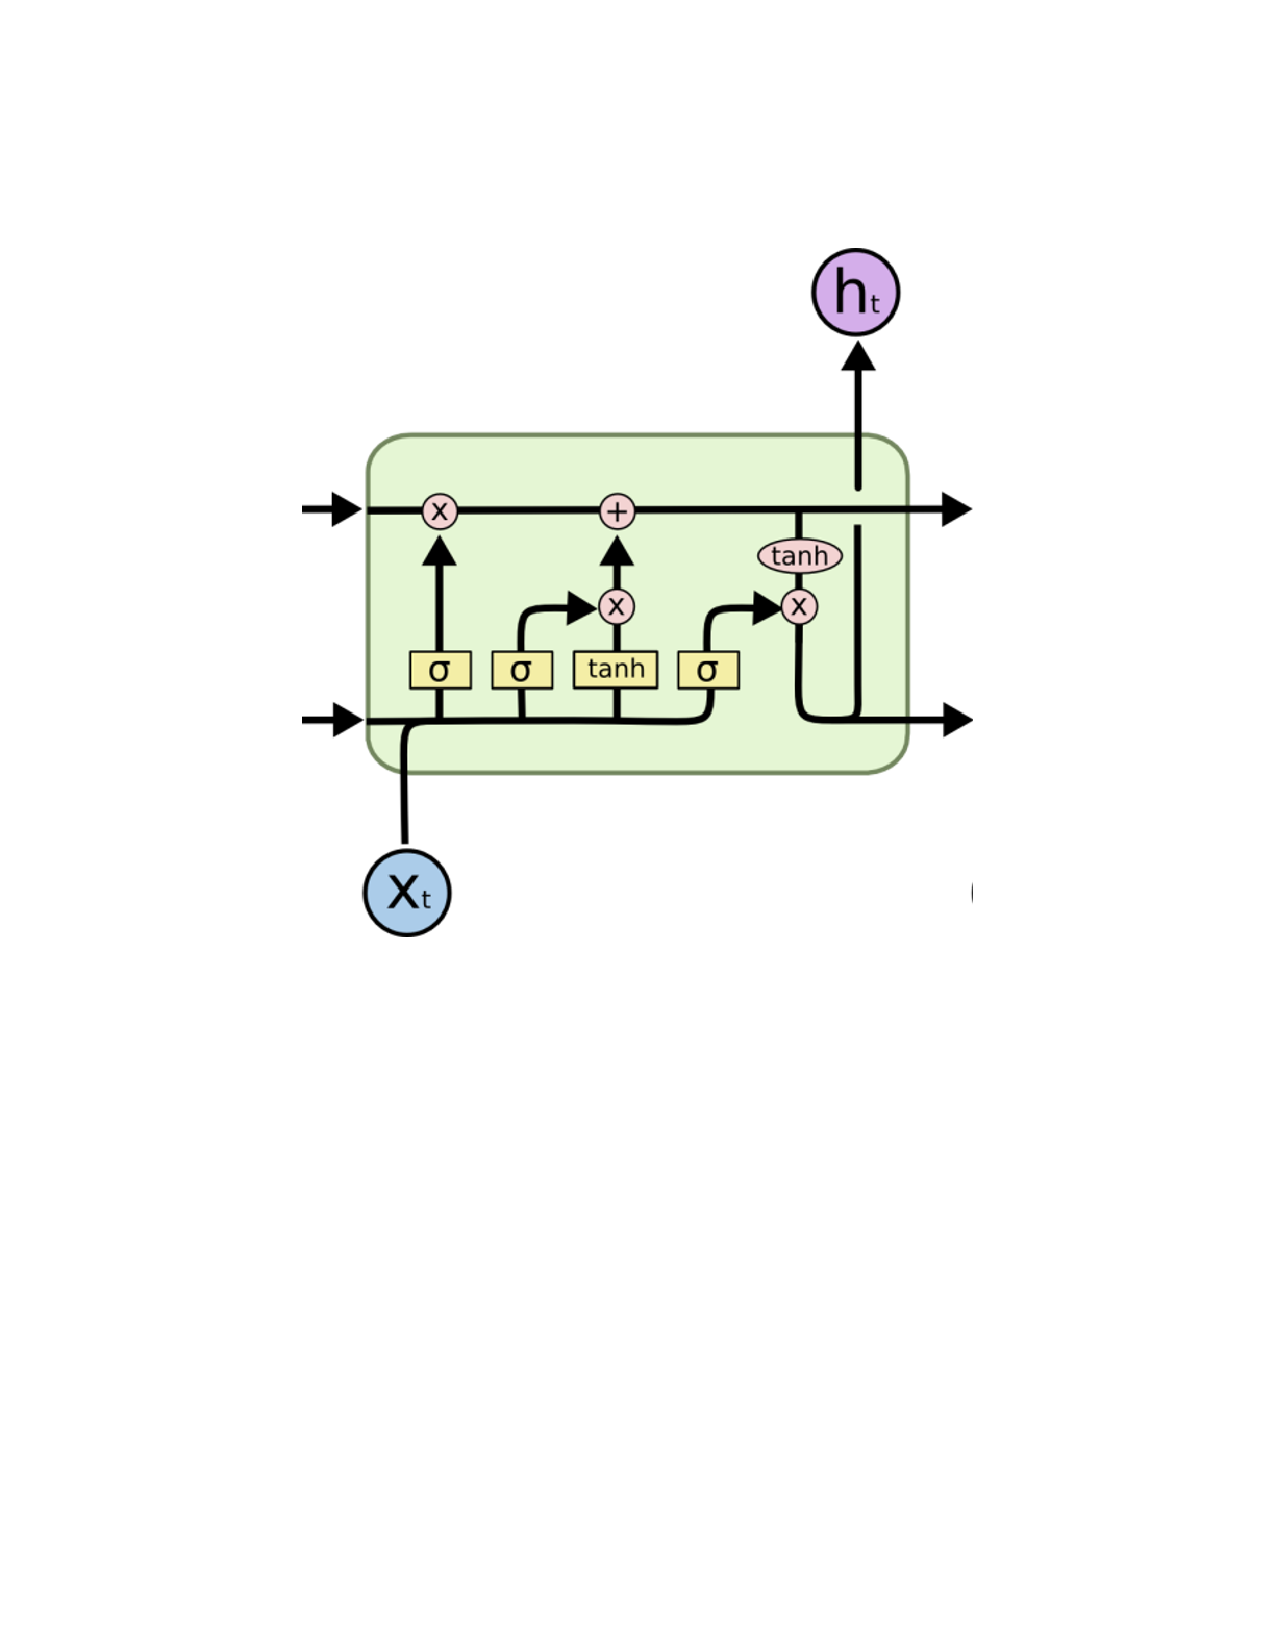
\includegraphics[width=6cm]{LSTM.pdf}
                % \caption{LSTM}
                % \label{LSTM_Cell_figures}
            \end{figure}
        \end{columns}
    \end{frame}

\section{My Methods and Methodology}
\subsection{dataset}
\begin{frame}{数据集}{xxxxx}
如表\ref{tab1}所示
\begin{table}
\centering
\caption{Dataset}
\label{tab1}
\begin{tabular}{cccccc}
\toprule
xx & xx & xx & xx & xx  \\
\midrule
0 & 0 & 0 & 18 & 0   \\
0  & 99 & 100 & 50 & 0  \\

\bottomrule
\end{tabular}
\end{table}
xxx rows-xxx cols
\end{frame}

\subsection{Review of Model}

\subsection{Details of Model}




\begin{frame}
    \begin{center}
        汇报完毕~~~~恳请指正
        ~\\
        ~\\
        ~\\
        ~\\
        ~\\
        Presented by
        ~\\
        xxx
    \end{center}
\end{frame}




\end{document}